\documentclass[conference]{IEEEtran}

% Language setting
% Replace `english' with e.g. `spanish' to change the document language
\usepackage[spanish]{babel}

% Useful packages
\usepackage{cite}
\usepackage{float}
\usepackage{graphicx}
\usepackage{url}

% Title and author info
\title{Desarrollo de una Pokédex con Comandos de Voz}
\author{\IEEEauthorblockN{Michael Rodriguez Rios}}

\begin{document}
\maketitle

\begin{abstract}
Este documento presenta el proceso de desarrollo de una Pokédex interactiva con capacidad de reconocimiento de voz para la búsqueda de Pokémon. Se utilizaron tecnologías web como HTML, CSS, JavaScript y las bibliotecas Artyom.js y jQuery. El objetivo principal fue crear una experiencia de usuario moderna y accesible para los entusiastas de Pokémon.
\end{abstract}

\section{Introduction}

La Pokédex es una herramienta esencial para los entrenadores de Pokémon, ya que proporciona información detallada sobre cada especie. En este proyecto, se desarrolló una Pokédex interactiva con una interfaz gráfica atractiva y la capacidad de realizar búsquedas utilizando comandos de voz. Esto permitió una experiencia de usuario más inmersiva y accesible.

\section{Desarrollo}
La implementación de la Pokédex se realizó utilizando HTML5, CSS3 y JavaScript, con la biblioteca jQuery para manipulación del DOM y llamadas AJAX, Bootstrap para diseño responsivo, y Artyom.js para añadir funcionalidad de reconocimiento de voz.
    
\subsection{Procedimiento}
\subsubsection{Interfaz gráfica}
En la Figura \ref{fig:interfaz} se presenta la interfaz desarrollada.
\begin{figure}[H]
    \centering
    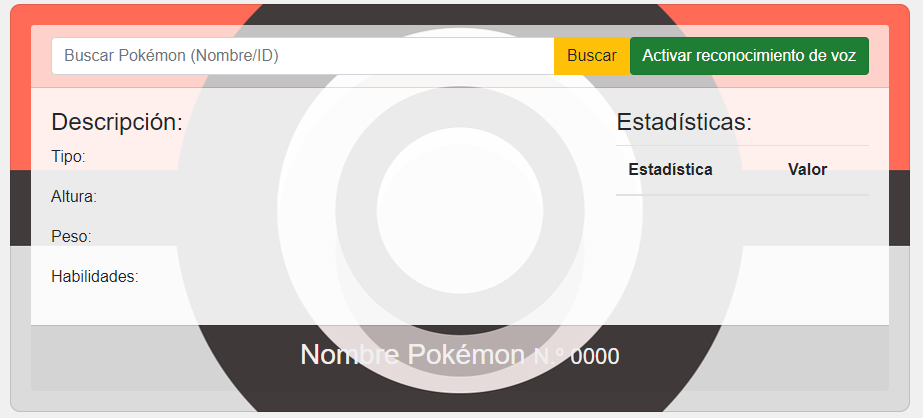
\includegraphics[width=0.8\columnwidth]{Interfaz.png}
    \caption{Interfaz gráfica de la Pokédex.}
    \label{fig:interfaz}
\end{figure}

\subsubsection{Búsqueda por nombre}
La interfaz permite realizar búsquedas por nombre del Pokémon como se evidencia en la Figura \ref{fig:busqueda-nombre}.
\begin{figure}[H]
    \centering
    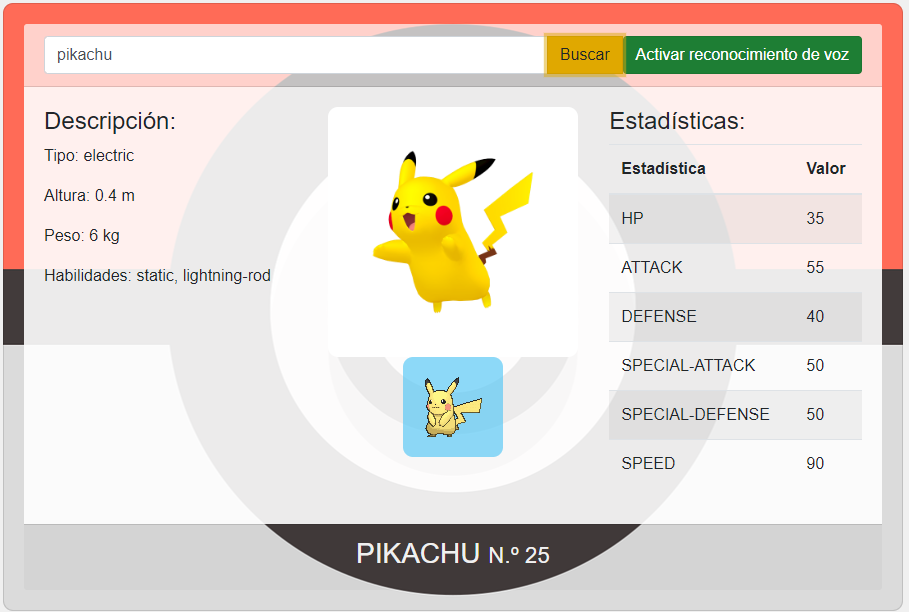
\includegraphics[width=0.8\columnwidth]{Busqueda-nombre.png}
    \caption{Búsqueda por nombre en cuadro de texto.}
    \label{fig:busqueda-nombre}
\end{figure}

\subsubsection{Búsqueda por ID}
La interfaz permite realizar búsquedas por ID del Pokémon como se evidencia en la Figura \ref{fig:busqueda-id}.
\begin{figure}[H]
    \centering
    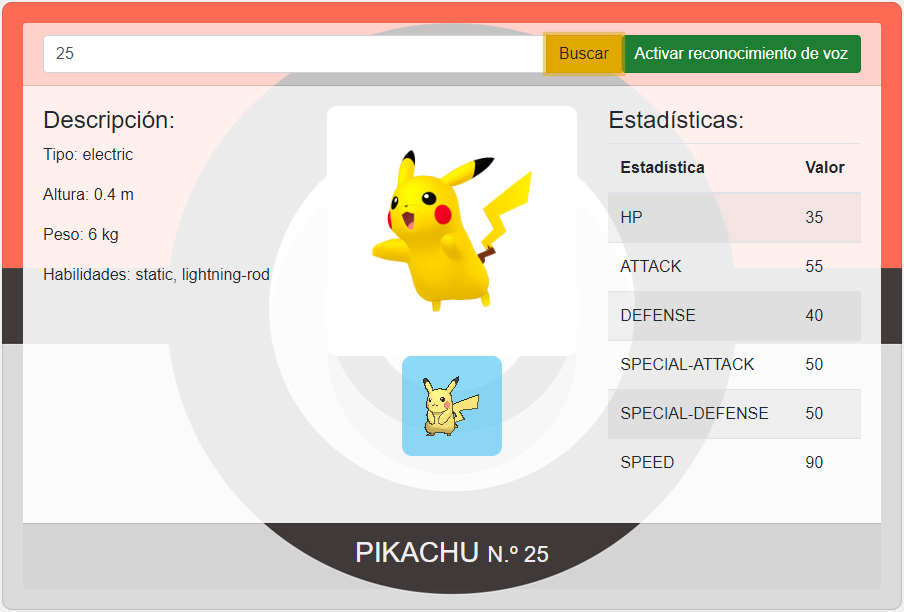
\includegraphics[width=0.8\columnwidth]{Busqueda-id.png}
    \caption{Búsqueda por ID en cuadro de texto.}
    \label{fig:busqueda-id}
\end{figure}


\section{Resultados}
La Pokédex desarrollada cuenta con las siguientes características:
\begin{itemize}
    \item Interfaz gráfica responsive desarrollada con HTML, CSS y Bootstrap\cite{bootstrap}.
    \item Consumo de datos de la API PokeAPI.co\cite{PokeAPI} utilizando JavaScript y AJAX.
    \item Integración de reconocimiento de voz con la biblioteca Artyom.js \cite{artyomjs}.
    \item Utilización de jQuery \cite{jquery} para la manipulación del DOM y las interacciones con la interfaz de usuario.
    \item Visualización de información detallada del Pokémon, incluyendo nombre, tipo, altura, peso, habilidades, estadísticas y sprites animados.\cite{PokeAPI}
    \item Manejo de errores en caso de que el Pokémon buscado no exista.
\end{itemize}

\section{Conclusiones}
La implementación de capacidades de reconocimiento de voz en la Pokédex ha resultado ser una estrategia interesante que promueve la interacción en la experiencia de los usuarios. Los resultados obtenidos sugieren un camino prometedor hacia la incorporación de interfaces de voz más avanzadas en aplicaciones web que faciliten el uso del softare por usuarios inexpertos.

\bibliographystyle{IEEEtran}
\bibliography{references}

% Fin del documento
\end{document}